%%%%%%%%%%%%%%%%%%%%%%%%%%%%%%%%%%%%%%%%%%%%%%%%%%%%%%%%%%%%%%%%%%%%
%%%% LVF_iclr2015_v1.tex file
%%%% Authors: Michael Giering, Kishore Reddy, Vivek Venugopalan
%%%% adapted from iclr2015.tex
%%%% v1 12-15-2014 13:35:11
%%%%%%%%%%%%%%%%%%%%%%%%%%%%%%%%%%%%%%%%%%%%%%%%%%%%%%%%%%%%%%%%%%%

\documentclass{article}
\usepackage{iclr2015,times} 
\usepackage{hyperref}
\usepackage{url}
\usepackage[pdftex]{graphicx}
\usepackage{amsfonts,amsmath,amssymb}
\usepackage{fixltx2e} % Fixing numbering problem when using figure/table* 
\usepackage{gensymb}
\usepackage{subfigure}

\title{Multi-modal Sensor Registration for Vehicle Perception via Deep Neural Networks}

\author{Michael Giering, Kishore Reddy, Vivek Venugopalan\\
Decision Support \& Machine Intelligence Group \\
United Technologies Research Center\\
E. Hartford, CT 06060, USA \\
Email: \{gierinmj, kkreddy, venugov\}@utrc.utc.com}


\newcommand{\fix}{\marginpar{FIX}}
\newcommand{\new}{\marginpar{NEW}}

\iclrconference
\begin{document}


\maketitle

\begin{abstract}

The ability to simultaneously leverage multiple modes of sensor information is critical for perception of an automated vehicle's physical surroundings. Spatio-temporal alignment of registration of the incoming information is often a prerequisite to analyzing the fused data. The persistence and reliability of multi-modal registration is therefore the key to the stability of decision support systems ingesting the fused information. LiDAR-video systems like on those many driverless cars are a common example of where keeping the LiDAR and video channels registered to common physical features is important. We develop a deep learning method that takes multiple channels of heterogeneous data, to detect the misalignment of the LiDAR-video inputs.  A number of variations were tested on the Ford LiDAR-video driving test data set and will be discussed. To the best of our knowledge the use of multi-modal deep convolutional neural networks for dynamic real-time LiDAR-video registration has not been presented.

\end{abstract}

%%%%%%%%%%%%%%%%%%%%%%%%%%%%%%%%%%%%%%%%%%%%%%%%%%%%%%%%
\section{Motivation} % (fold)
\label{sec:motivation}
% please include other motivations
Navigation and situational awareness of optionally manned vehicles requires the integration of multiple sensing modalities such as Light Detection and Ranging (LiDAR) and video, but could just as easily be extended to other modalities including Radio Detection And Ranging (RADAR), Short-Wavelength Infrared (SWIR) and Global Positioning System (GPS). Spatio-temporal registration of information from multi-modal sensors is technically challenging in its own right. For many tasks such as pedestrian and object detection tasks that make use of multiple sensors, decision support methods rest on the assumption of proper registration. Most approaches \cite{Bodensteiner2012Real-time-} in LiDAR-video for instance, build separate vision and LiDAR feature extraction methods and identify common anchor points in both. Alternatively, by generating a single feature set on LiDAR, Video and optical flow, it enables the system to to capture mutual information among modalities more efficiently. The ability to dynamically register information from the available data channels for perception related tasks can alleviate the need for anchor points \emph{between} sensor modalities. We see auto-registration as a prerequisite need for operating on multi-modal information with confidence.

%better fusion
Deep neural networks lend themselves in a seamless manner for data fusion on time series data. It has been shown [\cite{Ngiam2011Multimodal}] for some challenges in which the modalities share significant mutual information, the features generated on the fused information can provide insight that neither input alone can. In effect the ML version of, "the whole is greater than the sum of it's parts". 

%speed constraints
<<<<<<< HEAD
Autonomous navigation places significant constraints on the speed of perception algorithms and their ability to drive decision making in real-time. Though computationally intensive to train, the run time speed of our implemented Deep Convolutional Neural Networks (DCNN's) run easily within real-time frame rates of \textbf{60 fps???}. 

=======
Autonomous navigation places significant constraints on the speed of perception algorithms and their ability to drive decision making in real-time. Though computationally intensive to train, the run time speed of our implemented DCNN's run easily within real-time frame rates of \textbf{60 fps???}. 
>>>>>>> origin/master
%Applied research perspective
With most research in deep neural networks focused on algorithmic improvements and novel applications, a significant benefit to applied researchers is sometimes under appreciated. Feature generation
as executed in DNNs enables us to create such systems with far less overhead. The need for domain experts and hand-crafted feature design are lessened, allowing more rapid prototyping and testing. 
%%probably in next steps
The generalization of auto-registration across multiple assets is clearly a path to be explored. 

In this paper, the main contributions are: (i) formulation of an image registration problem as a fusion of modalities from different sensors, namely LIDAR (L), video (Grayscale or R,G,B) and optical flow (U,V); (ii) performance evaluation of DCNN with various input parameters, such as kernel filter size and different combinations of input channels (R,G,B,Gr,L,U,V); (iii) fusion of patch-level and image-level predictions to generate alignment at the frame-level. The experiments were conducted using a publicly available dataset from FORD and the University of Michigan [\cite{Pandey2011Ford-Campu}]. The DCNN implementation was targeted on a NVIDIA Tesla K40 GPU with 2880 cores and compute power of 5 TFLOPS (single precision). The paper is organized into the following sections: Section \ref{sec:motivation} describes the introduction and motivation for this work; Section \ref{sec:previous_work} provides a survey of the related work; the problem formulation along with the dataset description and the preprocessing is explained in Section \ref{sec:problem_statement}; Section \ref{sec:model_description} gives the details of the DCNN setup for the different experiments; Section \ref{sec:experiments_and_post_processing} describes the experiments and the post-processing steps for visualizing the qualitative results; finally Section \ref{sec:conclusions_and_future_work} summarizes the paper and conludes with future research thrusts.

% section motivation (end)

%%%%%%%%%%%%%%%%%%%%%%%%%%%%%%%%%%%%%%%%%%%%%%%%%%%%%%%%
\section{Previous Work} % (fold)
\label{sec:previous_work}
%% image registration
Kishore here

%%Multi-modal data fusion
A great amount has been published on various multi-modal fusion methods.\textbf{ insert new references here.}The most common approaches taken generate features of interest in each modality separately and create a decision support mechanism that aggregates features across modalities. If spatial alignment is required across modalities, as it is for LiDAR-video such filter methods \cite{Thrun2011Googles-dr} are required to ensure proper inter-modal registration. These filter methods for leveraging 3D LiDAR and 2D images are often geometric in nature and make use of projections between the different data spaces. 



%%deep learning multi-modal data fusion with CNN's

The use of deep neural networks to analyze multimodal sensor inputs  has increased sharply in the last couple of years, including audo-video \cite{Ngiam2011Multimodal} \cite{Kim2013Deep-Learn}, image/text \cite{Srivastava2012Multimodal}, image/depth \cite{Lenz2013Deep-Learn} and LiDAR-video To the best of our knowledge the use of multi-modal deep neural networks for dynamic real time LiDAR-video registration has not been presented.

A common question often arises in data fusion methods, which is "at what level should features from the differing sensor streams be brought together?" Most similar to the more traditional data fusion methods is to train DNN's independently on sensor modalities and then use the high-level outputs of those networks as inputs to a subsequent deep neural network This is analogous to the earlier example of learning 3D/2D features and subsequently identifying common geometric features. 

It is possible however to apply DNN's with a more agnostic view enabling a unified set of features to be learned across multi-modal data. In these cases the input channels aren't differentiated. Unsupervised methods in particular applying DBM's for learning such joint representations have been successful.  

DCNN's enable a similar agnostic approach to input channels. A significant difference is that target data is required to train them as classifiers. This is the approach chosen by us for automating the registration of LiDAR-video and optical-flow, in which we are combining 1D/3D/2D data representations to learn a unified model across as many as 6D. 


% section previous_work (end)


%%%%%%%%%%%%%%%%%%%%%%%%%%%%%%%%%%%%%%%%%%%%%%%%%%%%%%%%
\section{Problem Statement} % (fold)
\label{sec:problem_statement}

Being able to detect and correct the misalignment (registration, calibration) among sensors of the same or different kinds is critical when operating on the fused information emanating from them. For this work Deep Convolutional Neural Networks (DCNN) were implemented for the detection of small spatial misalignments in LiDAR and Video frames. The data collected from a driverless car was chosen as the multi-modal fusion test case. LiDAR-video is a common combination for providing perception capabilities to many types of ground and airborne platforms including driverless cars \cite{Thrun2011Googles-dr}. 

\subsection{Ford LiDAR-video Dataset and Experimental Setup} % (fold)
\label{sub:ford_lidar_video_dataset_and_experimental_setup}

\begin{figure}[htbp]
    \centering
        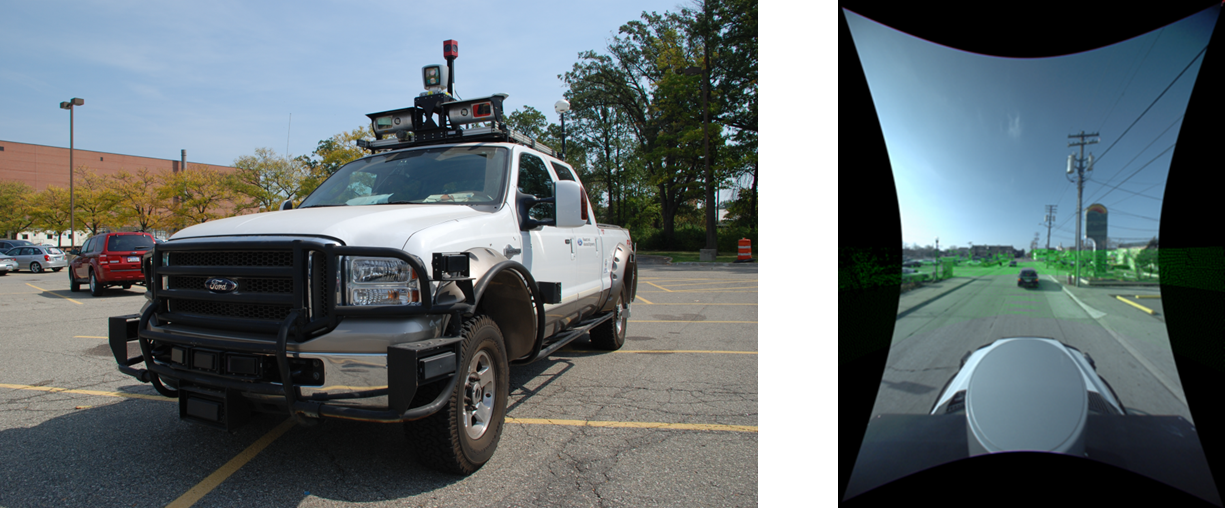
\includegraphics[scale=0.45]{Figures/ford-truck-sensors-final.png}
    \caption{Left: The modified Ford F-250 pickup truck. Right: Sample image from front facing camera and green dots indicate the region of LiDAR data.}
    \label{fig:ford-truck-sensors}
\end{figure}

The FORD LiDAR-video dataset \cite{Pandey2011Ford-campu} is collected by an autonomous Ford F-250 vehicle integrated with the following perception and navigation sensors as shown in Figure \ref{fig:ford-truck-sensors}:
\begin{itemize}
    \item Velodyne HDL-64E LiDAR with two blocks of lasers spinning at 10 Hz and a maximum range of 120m.
    \item Point Grey Ladybug3 omni-directional camera system with six 2-Mega-pixel cameras collecting video data at 8fps with $1600\times1600$ resolution.
    \item Two Riegl LMS-Q120 LIDAR sensors installed in the front of the vehicle generating range and intensity data when the laser sweeps its 80\degree field of view (FOV).
    \item Applanix POS-LV420 INS with Trimble GPS system providing the 6 degrees of freedom (DOF) estimates at 100 Hz.
    \item Xsens MTi-G sensor consisting of accelerometer, gyroscope, magnetometer, integrated GPS receiver, static pressure sensor and temperature sensor. It measures the GPS co-ordinates of the vehicle and also provides the 3D velocity and 3D rate of turn.
\end{itemize}

\begin{figure}[htbp]
    \centering
        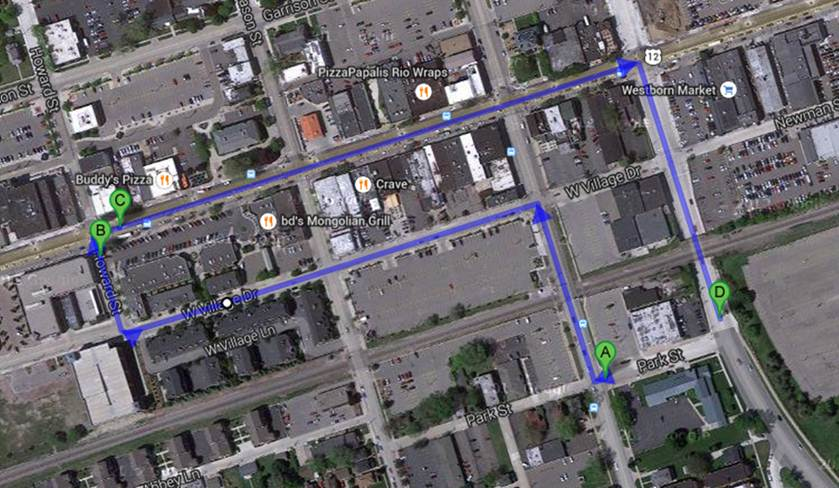
\includegraphics[scale=0.35]{Figures/ford_train_test_track.jpg}
    \caption{Training (A to B) and testing (C to D) tracks in the downtown Dearborn Michigan.}
    \label{fig:ford_train_test_track}
\end{figure}

This dataset is generated by the vehicle while driving in and around the Ford research campus and downtown Michigan. The data includes feature rich downtown areas as well as featureless empty parking lots. As shown in Figure \ref{fig:ford_train_test_track}, we divided the data set into training and testing sections A to B and C to D respectively. They were chosen in a manner that minimizes the likelihood of contamination between training and testing. Because of this, the direction of the light source is never the same in the testing and training sets. %If our methods are generalizable, they should be able to overcome this bias in the data.   

% subsection ford_LiDAR_video_dataset_and_experimental_setup (end)

\subsection{Optical Flow} % (fold)
\label{sub:optical_flow}

\begin{figure}[htbp]
    \centering
        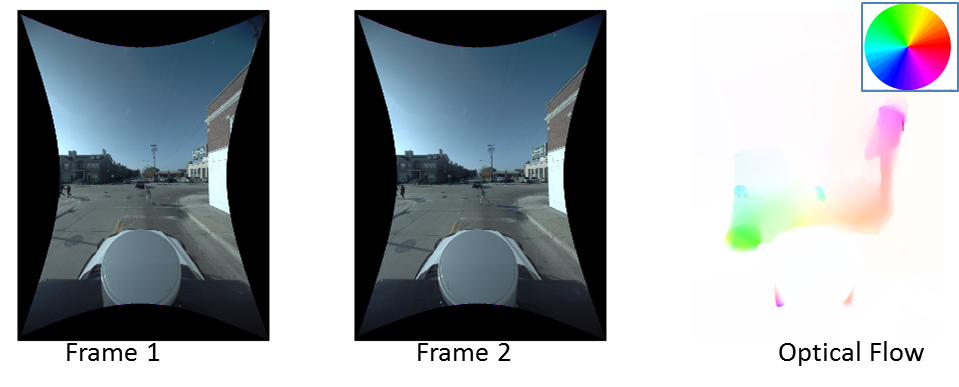
\includegraphics[scale=0.75]{Figures/OpticalFlow_example_final.png}
    \caption{Optical flow: Hue indicates orientation and saturation indicates magnitude}
    \label{fig:Figures_OptFlow placeholder}
\end{figure}

In the area of navigation of mobile robots, optical flow has been widely used to estimate egomotion [\cite{Prazdny1980-egomotion-OF}], depth maps [\cite{Shahraray1988-depthestimation-OF}], reconstruct dynamic 3D scene depth [\cite{Yang2012-reconstruction-OF}], and segment moving objects [\cite{Shao2002-seg-OF}]. Optical flow provides information of the scene dynamics and is expressed as an estimate of velocity at each pixel from two consecutive frames, denoted by $\vec{u}$ and $\vec{v}$. The motion field from these two frames is measured by the motion of the pixel brightness pattern, where the changes in image brightness is due to the camera or object motion. \cite{Liu2009Beyond-Pix} describes an algorithm for computing optical flow from images, which is used during the preprocessing step. Figure \ref{fig:Figures_OptFlow placeholder} shows an example of the optical flow computed using two consecutive frames from the Ford LiDAR-video dataset. By including optical flow as input channels, we imbue the DCNN with information on the dynamics observed across time steps.

% subsection optical_flow (end)

\subsection{Preprocessing} % (fold)
\label{sub:preprocessing}
%image of LiDAR-video-optical flow data with channels, patches and images(frames) denoted.
At each video frame timestep, the inputs to our model consist of \emph{C} channels of data with \emph{C} ranging from 3-6 channels. Channels consist of grayscale \emph{Gr} or \emph{(R,G,B)} information from the video, horizontal and vertical components of optical flow \emph{(U,V)} and depth information \emph{L} from LiDAR The data from each modality is reshaped to a fixed size of $800\times256$ values, which are partitioned into $p\times p$ patches at a prescribed stride. Each patch $p\times p$ is stacked across \emph{C} channels, effectively generating a vector of \emph{C} dimensions. The different preprocessing parameters are denoted by patch size \emph{p}, stride \emph{s} and the number of input channels \emph{C}.

Preprocessing is repeated \emph{N} times, where \emph{N} is the number of offset classes. For each offset class, the video (R,G,B) and optical flow (U,V) channels are kept static and the depth (L) channel from the LiDAR is moved by the offset simulating a misalignment between the video and the LiDAR sensors. In order to accurately detect the misalignment in the LiDAR and Video sensor data, a threshold is set to limit the information available in each channel. The LiDAR data has regions of sparsity and hence the LiDAR patches with a variance (${\sigma}^2 < 15\%$) are dropped from the final dataset. This leads to the elimination of the majority of foreground patches in the data set, reducing the size of the training and testing set by approximately 80\%. Figure \ref{fig:Figures_Ellipse} shows a $N = 9$ class elliptically distributed set of offsets and Figure \ref{fig:ImageChStride} shows a $p\times p$ patch stacked across all the different \emph{C} channels.

\begin{figure}[htbp]
    \centering
    \subfigure[Visualization of the elliptically distributed $N=9$ classes]
    {
        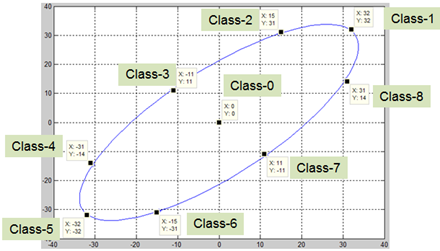
\includegraphics[scale=0.85]{Figures/ellipse.png}
        \label{fig:Figures_Ellipse}
    }
    \hspace{0.5cm}
    \subfigure[Stacking of $p\times p$ patch over all the different channels]
    {
        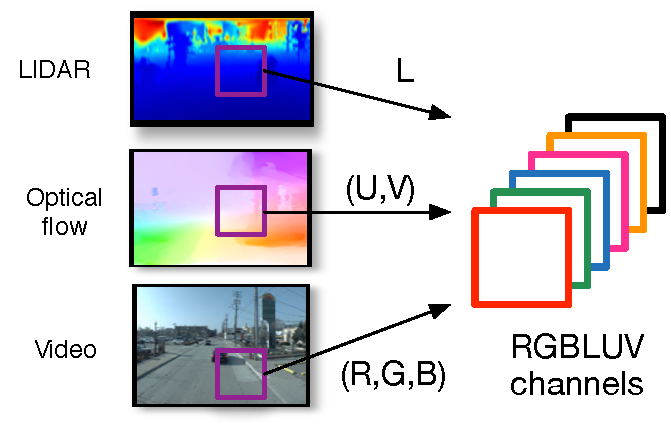
\includegraphics[scale=0.5]{Figures/ImagePatchChannel.pdf}
        \label{fig:ImageChStride}
    }
    \caption{Preprocessing steps}
    \label{fig:preprocessing_steps}
\end{figure}

% subsection preprocessing (end)

% section problem_statement (end)

%%%%%%%%%%%%%%%%%%%%%%%%%%%%%%%%%%%%%%%%%%%%%%%%%%%%%%%%
\section{Model Description} % (fold)
\label{sec:model_description}

\textbf{need to describe the parameters post-processing,classification metric for each patch,a table with common parameters for the experiments would help,voting scheme}

Our models for auto-registration are DCNN's trained to classify the current misalignment of the LiDAR-video data streams into one of a predefined set of offsets. DCNN's are probably the most successful deep learning model to date on fielded applications. The fact that the algorithm shares weights in the training phase, results in fewer model parameters and more efficient training. DCNN's are particularly useful for problems in which local structure is important, such as object recognition in images and temporal information for voice recognition. The alternating steps of convolution and pooling \textbf{(as depicted in figure X)}  generates features at multiple scales which in turn imbues DCNN's with scale invariant characteristics.


The model consists of a 4-layer \textbf{?} CNN classifier \textit{see image of network} that estimates the offset between the LiDAR-video inputs at each time step. For each patch within a timestep, there are O variants with the LiDAR-video-optical flow inputs offset by the predetermined amounts. The CNN outputs to a softmax layer, thereby providing an offset classification value for each patch of the frame. 
% figure of the colored class choices for the 5 class data set
figure x: In the 5 class example we color each patch of the frame with a color corresponding to the predicted class. 

For each frame a simple voting scheme is used to aggregate the patch level offset predictions to frame level predictions. A sample histogram of the patch level predictions is show in figure x.


% section model_description (end)

%%%%%%%%%%%%%%%%%%%%%%%%%%%%%%%%%%%%%%%%%%%%%%%%%%%%%%%%

\section{Experiments and Post-processing} % (fold)
\label{sec:experiments_and_post_processing}

The NVIDIA Kepler series K40 GPUs [\cite{NVIDIA-Inc.2012NVIDIAs-Ne}] are very FLOPS/Watt efficient and are being used to drive real-time image processing capabilities [\cite{Venugopal2013Accelerati}]. These GPUs consist of 2880 cores with 12 GB of on-board device memory (RAM). Deep Learning applications have been targeted on GPUs previously in [\cite{Krizhevsky2012Imagenet-C}] and these implementations are memory bound. A GPU with higher memory capacity is excellent for these experiments due to the number of channels that are stacked and provided as the input to the DCNN. The LiDAR-video dataset is augmented with the optical flow information resulting in 6 channels which means that the input to the DCNN is $32\times32\times6$ per patch. Figure \ref{fig:Figures_lidar_dcnn_setup1} shows the setup used for the DCNN implementation on the GPU, where \emph{C} defines the number of channels.

\begin{figure}[htbp]
    \centering
        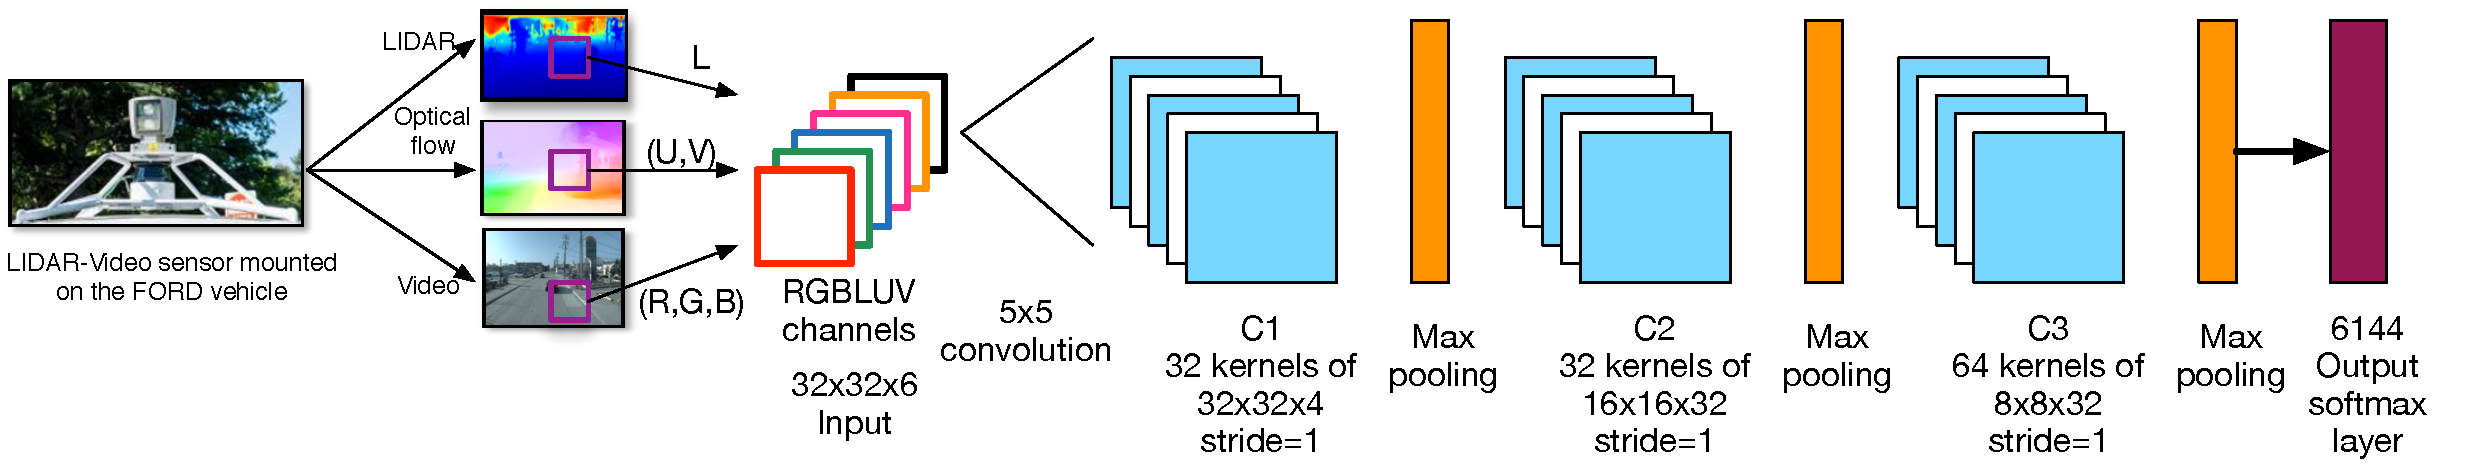
\includegraphics[scale=0.35]{Figures/lidar_dcnn_setup1.pdf}
    \caption{Experimental setup of the LiDAR-video DCNN with $5\times5$ convolution}
    \label{fig:Figures_lidar_dcnn_setup1}
\end{figure}

\textit{Need a complete list of the experiments run
images to visualize the frame level results
please place any confusion matrices and your comments on what you think the results say.
feel free to suggest any tables or other visuals to include.}




\subsection{5 class tests} % (fold)
\label{sub:5_class_tests}
% require a table of the different parameter settings, along with some aggregate measures from the confusion matrices. 
In our initial tests, the linearly distributed set of 5 offsets of the LiDAR-video data were performed. Table 1 lists the inputs and CNN parameters explored ranked in the order of increasing accuracy \textbf{(define accuracy and other cm metrics), include training vs test error and conf mats if room allows}.  

As can be seen ... 
% subsection 5_class_tests (end)


\subsection{9 class tests} % (fold)
\label{sub:9_class_tests}
% require a table of the different parameter settings, along with some aggregate measures from the confusion matrices. 
The subsequent tests were designed to understand whether the simple linear displacement model of the 5-class test could be generalized to a model capable of discriminating multiple directions and displacement magnitude. To achieve this 8 positions were chosen on an ellipse along with it's center \textbf{describe the parabola}. LiDAR-video was offset in a manner similar to the 5 class test. Nine training and test sets were generated and an identical patch level CNN was constructed differing only in the 9 class softmax output layer. 

\begin{figure}[htbp]
    \centering
        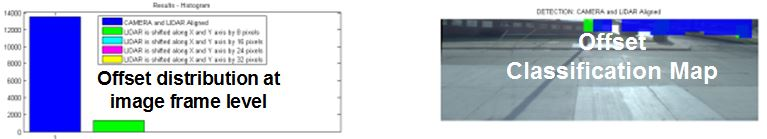
\includegraphics[scale=0.85]{Figures/Voting_5class.jpg}
    \caption{Placeholder: Voting}
    \label{fig:Figures_Voting}
\end{figure}

Table 2 lists the inputs and CNN parameters explored ranked in the order of increasing accuracy \textbf{(define accuracy and other cm metrics), include training vs test error and conf mats if room allows}.  

 \textbf{Discussion: what results confirmed expectations or surprised us (grey scale). Can we confidently say optical flow improves prediction. }
% subsection 9_class_tests (end)

% section experiments_and_post_processing (end)


%%%%%%%%%%%%%%%%%%%%%%%%%%%%%%%%%%%%%%%%%%%%%%%%%%%%%%%%
\section{Conclusions and Future Work} % (fold)
\label{sec:conclusions_and_future_work}
We did it. We're great.

%future: 
The next step in taking this work forward is to complete our development of a deep auto-registration method for ground and airborn platforms requiring no apriori calibration ground truth.  Our airborne applications in particular present nosier data with an increased number of degrees of freedom. The extension of these methods to simultaneously register information across multiple platforms and larger numbers of modalities will provide interesting challenges that we look forward to working on. 

% section conclusions_and_future_work (end)


%%%%%%%%%%%%%%%%%%%%%%%%%%%%%%%%%%%%%%%%%%%%%%%%%%%%%%%%
%\section{references}

\bibliographystyle{iclr2015}
\bibliography{references}

\end{document}
=======
>>>>>>> External Changes
=======
>>>>>>> External Changes
